\documentclass[12pt,a4paper]{article}

\usepackage[utf8]{inputenc}
\usepackage[greek,english]{babel}
\usepackage{alphabeta} 

\usepackage[pdftex]{graphicx}
\usepackage[top=1in, bottom=1in, left=1in, right=1in]{geometry}

\linespread{1.06}
\setlength{\parskip}{8pt plus2pt minus2pt}

\widowpenalty 10000
\clubpenalty 10000

\newcommand{\eat}[1]{}
\newcommand{\HRule}{\rule{\linewidth}{0.5mm}}

\usepackage[official]{eurosym}
\usepackage{enumitem}
\setlist{nolistsep,noitemsep}
\usepackage[hidelinks]{hyperref}
\usepackage{cite}
\usepackage{lipsum}


\begin{document}

%===========================================================
\begin{titlepage}
\begin{center}

% Top 

\includegraphics[width=0.3\textwidth]{images/Picture2.jpg}~\\[2cm]


% Title
\HRule \\[0.4cm]
{ \LARGE 
  \textbf{Mobile and Wireless Networking }\\[0.4cm] 
  \textbf{ITCE450-417 ITNE360}\\[0.4cm]
  \emph{Lab1 : Introduction to MATLAB}\\[0.4cm]
  %  add 
}
\HRule \\[1.5cm]



% Author
% prepared by :
{ \large
  Ali Redha Ali Al Jufairi \\[0.1cm]
  \texttt{20195330}
}

{ \large
  Sayed Mohammed Baqer Adnan\\[0.1cm]
  \texttt{202001826}
}
\vfill

%\textsc{\Large Cyprus University of Technology}\\[0.4cm]
\textsc{\large Department of Information Technology,\\Computer Engineering }\\[0.4cm]


% Bottom
{\large \today}
 
\end{center}
\end{titlepage}


\newpage



%===========================================================
%===========================================================
%===========================================================
\section{Objectives}
% wrtie me a list of objectives for this lab which is introudction to matlab
\begin{itemize}
\item To learn how to install  MATLAB and use the portal.
\item To learn how to use MATLAB to solve simple problems.
\item  To learn how to use MATLAB to plot the graph of the cosine function using values of x ranging from 0 to and label the x- and y- accesses.
\end{itemize}

\section{Introduction}
MATLAB is a high-level language and interactive environment that enables you to perform computationally intensive tasks faster than with traditional programming languages such as C, C++, and Fortran. MATLAB allows matrix manipulations, plotting of functions and data, implementation of algorithms, creation of user interfaces, and interfacing with programs written in other languages, including C, C++,Java, Fortran, and Python.

\section{report tasks}

%number list of tasks 
\begin{enumerate}
\item Write a MATLAB function to compute the average (mean) of a vector x, then call and execute the function from the command window 
\begin{enumerate}
  \item Take a screenshot of the command.  
\end{enumerate}
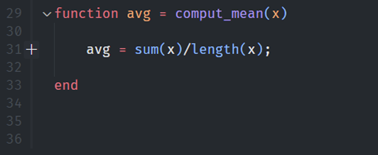
\includegraphics[width=0.8\textwidth]{images/Picture3.png}~\\[3cm]

\item  Take three screenshots for the output after calling the function with different Values of x.we wrote a simple function to generate a rand vector and then we called the function with the vector as an input and we got the mean of the vector as an output and for loop call 2 function and then printout .


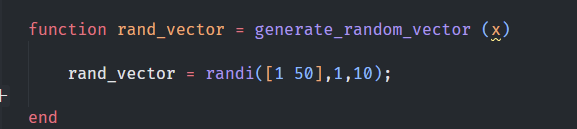
\includegraphics[width=0.8\textwidth]{images/Picture4.png}~\\[3cm]
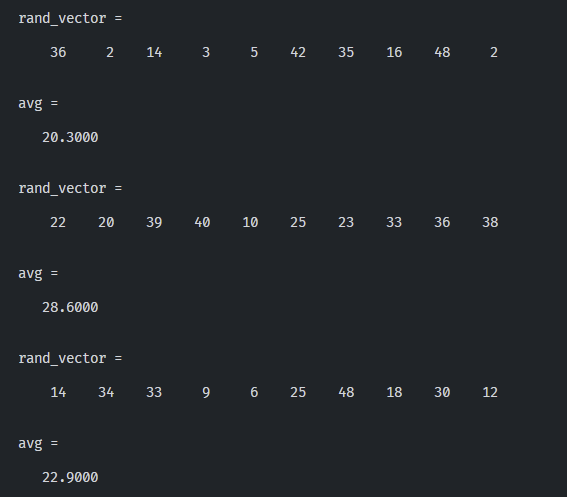
\includegraphics[width=0.8\textwidth]{images/Picture5.png}~\\[3cm]
\item Plot the graph of the cosine function using values of x ranging from 0 to and label the x- and y- accesses.
\begin{itemize}
  \item Add Labels for the x- and y- accesses.
  \item Add a title for your graph call it "Cosine Wave plot". 
  \item Add a grid
  \item Add a legend and call your result "Cosine Wave".
  \item Take a screenshot of your code and the cosine graph
\end{itemize}
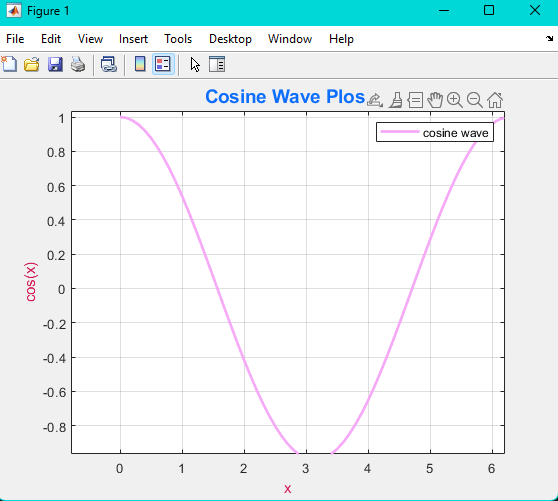
\includegraphics[width=0.8\textwidth]{images/Picture6.png}~\\[3cm]
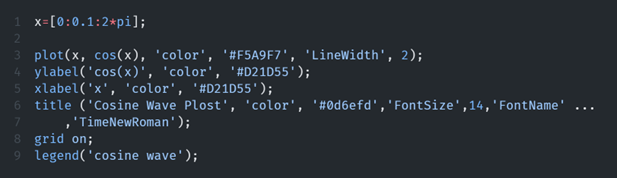
\includegraphics[width=0.8\textwidth]{images/Picture7.png}~\\[3cm]
\end{enumerate}

\section{Conclusion}
In this lab we learned how to use MATLAB to solve simple problems and we learned how to use MATLAB to plot the graph of the cosine function using values of x ranging from 0 to and label the x- and y- accesses.

%===========================================================
%===========================================================



\end{document} 
